%*******************************************************************************
%******************************** Chapter XXXXXXXX *****************************
%*******************************************************************************

\chapter{Introduction and Theory} \label{chap:Theory} %Title of chapter

\newcommand{\Dmq}{\Delta m^2}
\newcommand{\eVq}{\ensuremath{\text{eV}^2}}

\graphicspath{{Theory/Figs/Raster/}{Theory/Figs/PDF/}{Theory/Figs/Vector/}}

%%% Experiments
\nomenclature[z-SK]{SK}{Super-Kamiokande}

%%% Neutrino physics
\nomenclature[z-CP]{CP}{Charge-Parity}
\nomenclature[z-GUT]{GUT}{Grand Unified Theory}
\nomenclature[z-SM]{SM}{Standard Model}

%%% How LArTPCs work
\nomenclature[z-LAr]{LAr}{Liquid Argon}
\nomenclature[z-TPC]{TPC}{Time Projection Chamber}
\nomenclature[z-LArTPC]{LArTPC}{Liquid Argon Time Projection Chamber}

%%% SUSY
\nomenclature[z-SUSY]{SUSY}{SUperSYmmetry}
\nomenclature[z-MSSM]{MSSM}{Minimally Supersymmetric Standard Model}
\nomenclature[z-LSP]{LSP}{Lightest Supersymmetric Particle}

%%% An introduction to the standard model....
The ``Standard Model of Particle Physics'' (SM) is a set of theories which has been widely tested and has been found to accurately predict the interactions of fundamental particles. These tests have come in many forms throughout the 20$^{th}$ and 21$^{st}$ centuries, and include the detection of all of the quarks and leptons which it predicts, as well as measurements of the properties of these particles. The recent discovery of the Higgs boson~\citep{HiggsAtlas, HiggsCMS} ``completed'' the SM, as this was the last particle which it predicted to be observed. However, despite its many successes, the SM does not represent the ``final'' theory of fundamental particle physics, should one exist. This is because there are many questions made by recent experimental observations which the SM is unable to address, some of these will be briefly discussed below. \\

Firstly, though the SM accurately predicts the interactions made by the electromagnetic, weak nuclear, and strong nuclear forces, it makes no mention of gravity. This is a major flaw of the SM as gravity is one of the driving forces in the formation of astronomical objects such as planets, stars, and galaxies. With the recent detection of gravitational waves~\citep{LIGO} this issue has again be brought into focus. Secondly, the rotational velocities of galaxies is measured to be far greater than the predicted value, hinting at the presence of a significant amount of matter which we are unable to detect. The SM makes no prediction as to what this ``dark-matter'' is comprised of. Thirdly, measurements of distant supernovae appear to show that the expansion of the universe is accelerating, not decelerating as would be expected, this implies the presence of some form of unknown energy source. Again, the SM makes no prediction as to what this unknown energy source, or ``dark-energy'' is. A further point of consternation with the SM is that it is not ``elegant,'' as it has as many as 19 free parameters, which appear to be unrelated to each other. There are also unresolved questions regarding the particles which are predicted by the SM, such as, why charge is quantised, why there are exactly 3 families of quarks and leptons, and why they have the observed hierarchy of masses. The SM also does not predict the matter-antimatter asymmetry which is observed in the universe today. Finally, the neutrinos predicted by the SM are massless, however, numerous measurements of neutrino oscillations show that neutrinos should have a non-zero rest mass. A rigorous discussion of neutrino oscillations is presented in Section~\ref{sec:NeutPhys}. \\

Extensive efforts have been made to resolve many of these issues with the SM, in the form of a so-called Grand Unified Theory (GUT). These theories propose that the electroweak and strong nuclear forces belong to an overarching symmetry group. The unification of these forces is predicted to occur at extremely high energies, far beyond the reach of current experiments. As a result, many of the experimental signatures which these GUTs predict are difficult to measure. However, many GUTs predict that the proton, a stable particle in the SM, should decay with a lifetime of around 10$^{30-36}$ years, though some models predict much longer lifetimes. Some of the gauge groups which are invoked by GUTs are briefly discussed in Section~\ref{sec:Theory_NDK}, with reference to the proton lifetimes which they predict. A discussion of the backgrounds to proton decay searches is presented in Section~\ref{sec:BkNDK}. \\

The Deep Underground Neutrino Experiment (DUNE) is a next generation experiment to be built at the Sanford Underground Research Facility (SURF), which aims to measure many of the properties of neutrinos, as well as to search for nucleon decays. The experimental setup, physics capabilities, and prototyping schedule for DUNE are outlined in Chapter~\ref{chap:DUNE}. A camera system which was installed in the DUNE 35 ton prototype detector is described in Chapter~\ref{chap:Cameras}. Chapter~\ref{chap:35tonSim} describes simulations which were made in preparation for data taking of the 35 ton prototype, and conclude with a description of how Particle IDentification (PID) could be performed in the 35 ton data. An overview of the data gathered by the 35 ton prototype is shown in Chapter~\ref{chap:35tonData}, and a novel method of interaction time determination using the effects of diffusion is presented. Following this, Chapter~\ref{chap:FDSims} concerns simulations of the cosmogenic backgrounds seen in a large Liquid Argon Time Projection Chamber (LArTPC) at SURF. These simulations are first presented with respect to a surface detector measuring neutrino oscillations, and then to a detector at depth searching for nucleon decay events. Finally, Chapter~\ref{chap:Conc} contains some final remarks and observations. \\

%********************************** %First Section  **************************************
\section{Neutrino physics} ~\label{sec:NeutPhys}  %Section - X.1 
The study of neutrinos offers a chance to probe the limitations of the SM, as the neutrinos predicted by the SM are massless and do not oscillate. However, numerous measurements have shown that neutrino oscillations occur, and that at least two of the neutrino mass eigenstates have non-zero mass. Notably, the 2015 Nobel prize in physics was given to T. Kajita and A. McDonald for ``the discovery of neutrino oscillations, which shows that neutrinos have mass,'' based on their work on Super-Kamiokande (SK)~\citep{PhysRevLett.81.1562} and SNO~\citep{PhysRevLett.89.011301} respectively. This means that through studying neutrino oscillations, it is possible to begin to get a handle on physics beyond the SM. The history of the discovery of neutrino oscillations, which culminated in this Nobel prize, is briefly outlined in Section~\ref{Neut_Hist}. Following this, the formalism by which neutrino oscillations occur is presented in Section~\ref{Neut_Oscil}. Finally, the current state of neutrino physics, including the current best fit values for the various mixing parameters, is summarised in Section~\ref{sec:Theory_Exp}. \\

%%% The history
\subsection{The history of neutrino oscillations} \label{Neut_Hist}
Neutrinos were first proposed to explain the continuous energy spectrum of the electrons produced in $\beta$ decay, as due to kinematic constraints, it could not be explained by a two body decay. To this end, Pauli proposed the idea of a neutral particle, with mass less than that of the electron, which would not be observed in the reaction~\citep{Pauli}. Pauli called this particle a ``neutron.'' Upon the discovery that the ``neutron'' was in fact of a similar mass to the proton, and that the nucleus was a bound state of protons and neutrons, Fermi proposed a more complete theory of $\beta$ decay in 1934. In this theory, Fermi proposed that the light, neutral particle that was initially proposed by Pauli did exist, and was emitted from the nucleus in the reaction. Fermi called this particle a ``neutrino,'' meaning ``little neutral one'' in Italian. He also proposed that its mass could be measured by looking at the end point of the $\beta$ spectrum~\citep{Fermi:1934hr}. The first experiments designed to measure the neutrino mass in this way set an upper mass limit of 500 eV~\citep{NeutMassLim1, NeutMassLim2}, which was improved to 250 eV in the 1950's~\citep{NeutMassLim3}. After becoming evident that the neutrino mass was so much less than that of the electron, the idea that neutrinos were massless gained traction. \\

The first direct observation of neutrinos was in 1956~\citep{Cowan:1992xc}, and in 1962 conclusive proof emerged that the electron and muon neutrinos were distinct particles~\citep{PhysRevLett.9.36}. The experiment which found this, did so by observing that it was far more likely that the neutrinos produced in the decay of pions would interact to create muons, as opposed to electrons. This meant that there had to be two flavours of neutrinos, as if there was only a single flavour of neutrino, then when they should produce equal numbers of electrons and muons when they interact. However, soon after this an experiment by Ray Davis in 1968 at the Homestake Mine gave rise to the ``Solar neutrino problem''~\citep{RayDavis1968}. The Homestake experiment used a chlorine detector to look for the electron neutrinos produced by the sun, and measured a flux which was roughly $\frac{1}{3}$ of the predicted flux from solar models. The experiment ran for over 20 years, with the measured $v_{e}$ flux being unchanged at roughly $\frac{1}{3}$ of the predicted solar flux~\citep{RayDavis1988}. \\

The long standing observation that the solar $v_{e}$ flux was significantly lower than predicted, meant that either, there was some mechanism by which the electron neutrinos were evading detection, or that the solar model was incorrect. It was plausible that the solar model was incorrect, however the scale of the difference in the observed and predicted $v_{e}$ fluxes proved difficult to resolve. As a result, the idea of neutrino oscillation grew momentum, drawing on a prediction made by Pontecorvo as far back as 1957~\citep{Pontecorvo1957}. The Kamiokande-II experiment measured high energy solar neutrinos, and in 1989 measured an energy dependant deficit in the solar $v_{e}$ flux~\citep{PhysRevLett.63.16}. When studying the atmospheric neutrino flux, Kamiokande-II found an angular dependent deficit in the expected muon neutrino flux, though the electron neutrino flux was consistent with predictions. It was found that this deficit was consistent with oscillations of $\nu_{\mu} \leftrightarrow \nu_{\tau}$~\citep{PhysRevLett.81.1562}. The tau lepton, the third flavour of leptons, had been observed in the 1970s~\citep{PhysRevLett.35.1489}, though the $\nu_{\tau}$ neutrino was not directly measured until 2000~\citep{Kodama2001218}. \\

Conclusive proof for neutrino oscillations came in 2001, when the SNO experiment measured both the Neutral Current (NC) and Charged Current (CC) interactions of solar neutrinos. The SNO experiment measured a charge current interaction rate which was consistent with earlier experiments~\citep{Ahmad:2001an}, i.e. a deficit in the predicted solar flux. However, it found that the neutral current interaction rate, which is sensitive to all flavours of neutrinos, matched the predicted solar flux~\citep{PhysRevLett.89.011301}. This demonstrated that a significant part of the $v_{e}$ flux from the sun, had oscillated into $v_{\mu}$ and $v_{\tau}$ as they travelled to Earth. This flux of oscillated $v_{\mu}$ and $v_{\tau}$ could not interact via CC interactions, due to the high mass of the associated leptons relative to the neutrino energy, however, they are able to interact via NC interactions. \\

These highlighted results, as well as many other accompanying results, form the basis of our current understanding of neutrino oscillations. \\

%%% The formalism...
\subsection{The theory of neutrino oscillations} \label{Neut_Oscil}
Neutrino oscillations are described by the PMNS matrix, which is named after work initially done by Pontecorvo~\citep{Pontecorvo1957}, and then later extended by Maki, Nakagawa and Sakata~\citep{PMNS}. The PMNS matrix describes neutrino mixing in the context of the three known flavour states $\nu_e$, $\nu_\mu$ and $\nu_\tau$ being related to three neutrino mass states $\nu_1$, $\nu_2$ and $\nu_3$. This formalism then has the form shown in Equation~\ref{eq:PMNS_Short}.
\begin{equation}
  \label{eq:PMNS_Short}
  \begin{pmatrix} \nu_e \\ \nu_\mu \\ \nu_\tau \end{pmatrix} = U_{PMNS} \begin{pmatrix} \nu_1 \\ \nu_2 \\ \nu_3 \end{pmatrix}
\end{equation}
The matrix labelled $U_{PMNS}$ in Equation~\ref{eq:PMNS_Short}, is then expressed by Equations~\ref{eq:PMNS_El},~\ref{eq:PMNS_Who} and~\ref{eq:PMNS_Exp}. In these equations it has been assumed that $U_{PMNS}$ is unitary, and that there are three angles ($\theta_{12}$, $\theta_{13}$ and $\theta_{23}$) plus a CP-violating phase $\delta$, which explain the mixing between the mass and flavour eigenstates. The notation $s_{\alpha\beta}$ and $c_{\alpha\beta}$ has been used to denote $\sin\theta_{\alpha\beta}$ and $\cos\theta_{\alpha\beta}$ respectively. \\
\begin{align}
  U_{PMNS} &= \begin{pmatrix} U_{e1} & U_{e2} & U_{e3} \\ U_{\mu1} & U_{\mu2} & U_{\mu3} \\ U_{\tau1} & U_{\tau2} & U_{\tau3} \end{pmatrix} \label{eq:PMNS_El} \\
  &= \begin{pmatrix} c_{12}c_{13}                                  & s_{12}c_{13}                                  & s_{13}e^{-i\delta} \\
                     -s_{12}c_{23} - c_{12}s_{23}s_{13}e^{i\delta} & c_{12}c_{23} - s_{12}s_{23}s_{13}e^{i\delta}  & s_{23}c_{13}      \\
                     s_{12}s_{23} - c_{12}s_{23}s_{13}e^{i\delta}  & -c_{12}s_{23} - s_{12}c_{23}s_{13}e^{i\delta} & c_{23}c_{13}      \end{pmatrix} \label{eq:PMNS_Who}  \\
  &= \begin{pmatrix} 1 & 0 & 0                       \\ 0 & c_{23} & s_{23}  \\ 0 & -s_{23} & c_{23}            \end{pmatrix}
     \begin{pmatrix} c_{13} & 0 & s_{13}e^{-i\delta} \\ 0 & 1 & 0            \\ -s_{13}e^{i\delta} & 0 & c_{13} \end{pmatrix}
     \begin{pmatrix} c_{12} & s_{12} & 0             \\ -s_{12} & c_{12} & 0 \\ 0 & 0 & 1                       \end{pmatrix} \label{eq:PMNS_Exp}
\end{align}

Equation~\ref{eq:PMNS_El} shows how each element in the $U_{PMNS}$ relates the flavour states to the mass states, whilst Equation~\ref{eq:PMNS_Who} shows the full mixing formalism for Dirac neutrinos. Finally, Equation~\ref{eq:PMNS_Exp} separates the full formalism into three 3$\times$3 matrices which each contain one of the three mixing angles. \\

Should neutrinos be Majorana particles, then the $U_{PMNS}$ matrices should be multiplied by diag$\left(e^{i\alpha_1/2}, e^{i\alpha_2/2}, 1\right)$. The question of whether neutrinos are Majorana or Dirac particles does raise important questions for neutrino physics. This is because should neutrinos be Majorana particles, their masses could be generated via a Majorana mass term. There are next generation experiments such as SNO+~\citep{SNO+} and SuperNEMO~\citep{SuperNEMO}, which will search for neutrinoless double beta decay as a means to test whether neutrinos are Majorana particles. However, the two Majorana phases do not affect neutrino oscillations, and so will not be covered further in this discussion of neutrino oscillations. \\

This results in the neutrino mixing matrix being constrained by four independent parameters:
\begin{itemize}
 \item Three mixing angles ($\theta_{13}$, $\theta_{12}$, $\theta_{23}$).
 \item The CP-violating phase ($\delta$).
\end{itemize}

When neutrinos are produced and detected, we observe neutrinos of distinct flavour states, and not the distinct mass states. Therefore, a discussion of how mixing occurs will be presented in terms of an initial neutrino composed of a distinct flavour state, and multiple mass states. In this case a neutrino $\nu_\alpha$ will be produced, of flavour $\alpha$, which is a linear superposition of the three mass eigenstates $\nu_j$, such that $j=1,2,3$ (Equation~\ref{eq:Oscill_Eigen}). 
\begin{equation}
  \label{eq:Oscill_Eigen}
  \ket{\nu_\alpha} = \sum_{j}U^{\ast}_{\alpha j}\ket{\nu_j}
\end{equation}
where $U^{\ast}_{\alpha j}$ is one of the elements in Equation~\ref{eq:PMNS_El}. As this neutrino propagates, the mass eigenstates will evolve according to the time-dependant Schr\"{o}dinger equation, such that after time $t$, each mass eigenstate will have the form shown in Equation~\ref{eq:Oscill_MassProp1}.
\begin{equation}
  \label{eq:Oscill_MassProp1}
  \ket{\nu_j(t)} = e^{-i(E_{j}\cdot t - \vec{p_{j}}\cdot\vec{x_{j}})}\ket{\nu_j(0)}
\end{equation}
where assuming that the neutrino is ultra-relativistic, and setting $\hbar=c=1$:
\begin{align}
  t &\approx L \label{eq:Oscill_t2L} \\
  E &= \sqrt{p^2+m^2} = p \times \sqrt{1+\frac{m^2}{p^2}} \approx p + \frac{m^2}{2p} \approx p + \frac{m^2}{2E} \label{eq:Oscill_ESub} \\
  E_{j}\cdot t - \vec{p_{j}}\cdot\vec{x_{j}} &\approx \vec{p_{j}}L + \frac{m_{j}^2}{2E}L - \vec{p_{j}}L = \frac{m_{j}^2}{2E}L \label{eq:Oscill_FinSub}  
\end{align}
where a Taylor series expansion about $\sqrt{1+x^2}$ has been used in Equation~\ref{eq:Oscill_ESub}. Substituting Equation~\ref{eq:Oscill_FinSub} into Equation~\ref{eq:Oscill_MassProp1} gives Equation~\ref{eq:Oscill_MassProp2}.
\begin{equation}
  \label{eq:Oscill_MassProp2}
  \ket{\nu_j(t)} = e^{-im_{j}^{2}L/2E}\ket{\nu_j(0)}
\end{equation}
This then gives the time evolution of the original neutrino flavour state as Equation~\ref{eq:Oscill_TimeEigen}.
\begin{equation}
  \label{eq:Oscill_TimeEigen}
  \ket{\nu_\alpha(t)} = \sum_{j}U^{\ast}_{\alpha j}e^{-im_{j}^{2}L/2E}\ket{\nu_j(0)}
\end{equation}
From this, it can be seen that the mass states propagate with different phases, and so should the neutrino be detected at a later time it would exist as a superposition of different flavour states. This results in there being a non-zero possibility that the flavour of the neutrino which is detected, $\beta$, is not the same as the flavour with which the neutrino was produced with, $\alpha$. The amplitude with which this occurs is given by Equation~\ref{eq:Oscill_Amp}.
\begin{align}
    A(\nu_{\alpha}\rightarrow\nu_{\beta}) &= \bra{\nu_{\beta}}\ket{\nu_\alpha(t)} \nonumber \\
    &= \sum_{k}\sum_{j}\bra{\nu_{j}}U_{\beta j}U^{\ast}_{\alpha k}e^{-im_{k}^{2}L/2E}\ket{\nu_{k}} \nonumber \\
    &= \sum_{k}U^{\ast}_{\alpha k}U_{\beta k}e^{-im_{k}^{2}L/2E}   \label{eq:Oscill_Amp}
\end{align}
Equation~\ref{eq:Oscill_Amp}, can then be used to get the probability for the original neutrino $\nu_{\alpha}$ to oscillate to a different flavour $\nu_{\beta}$:
\begin{align}
  P(\nu_{\alpha}\rightarrow\nu_{\beta}) &= |\bra{\nu_{\beta}}\ket{\nu_\alpha(t)}|^2 \nonumber \\
  &= \left|\sum_{k}U^{\ast}_{\alpha k}U_{\beta k}e^{-im_{k}^{2}L/2E}\right|^2 \label{eq:Oscill_Prob1}\\
  &= \sum_{k}U^{\ast}_{\alpha k}U_{\beta k}e^{-im_{k}^{2}L/2E} \sum_{j}U^{\ast}_{\alpha j}U_{\beta j}e^{-im_{j}^{2}L/2E} \nonumber\\
  &= \sum_{k}\sum_{j}U^{\ast}_{\alpha k}U_{\beta k}U^{\ast}_{\alpha j}U_{\beta j}exp\left(-i\frac{(m^{2}_{k}-m^{2}_{j})L}{2E}\right) \label{eq:Oscill_Prob2}
\end{align}
The $(m^{2}_{k}-m^{2}_{j})$ term in Equation~\ref{eq:Oscill_Prob2} is often written as $\Delta m^{2}_{kj}$, and will be written as such for the remainder of the discussion of neutrino mixing. \\

In the interests of simplicity, an explicit calculation of the neutrino oscillation probability will be given assuming that there are only two neutrino flavour and mass states. The reason for this is that then there is only one mixing angle ($\theta$), and no complex phase. We are also free to choose the simplest mixing matrix, such that the mixing matrix becomes Equation~\ref{eq:PMNS_Simp}.
\begin{equation}
  \label{eq:PMNS_Simp}
  \begin{pmatrix} \nu_{\alpha} \\ \nu_{\beta} \end{pmatrix} = \begin{pmatrix} \cos\theta & \sin\theta \\ -\sin\theta & \cos\theta \end{pmatrix} \begin{pmatrix} \nu_1 \\ \nu_2 \end{pmatrix}
\end{equation}
The probability of a neutrino oscillating from initial flavour $\nu_{\alpha}$ to flavour $\nu_{\beta}$ is then given by Equation~\ref{eq:Oscil_TwoNeut}, which starts from Equation~\ref{eq:Oscill_Prob1}.
\begin{align}
  P(\nu_{\alpha}\rightarrow\nu_{\beta}) &= \left|(U_{\alpha 1}U_{\beta 1}e^{-im_{1}^{2}L/2E}) + (U_{\alpha 2}U_{\beta 2}e^{-im_{2}^{2}L/2E})\right|^2 \nonumber \\
  &= \left|(\cos\theta)(-\sin\theta)e^{-im_{1}^{2}L/2E} + (\sin\theta)(\cos\theta)e^{-im_{2}^{2}L/2E}\right|^2 \nonumber \\
  &= 2\cos^{2}\theta\sin^{2}\theta - \cos^{2}\theta\sin^{2}\theta\left[ e^{-i\frac{(m^{2}_{1}-m^{2}_{2})L}{2E}} + e^{-i\frac{(m^{2}_{2}-m^{2}_{1})L}{2E}} \right] \nonumber\\ 
  &\text{using $\cos\left(\phi_1 - \phi_2\right) = \left(e^{i(\phi_1-\phi_2)} + e^{-i(\phi_1-\phi_2)}\right)/2$} \nonumber \\
  &= 2\cos^{2}\theta\sin^{2}\theta - \cos^{2}\theta\sin^{2}\theta\left[ 2\cos\left(\frac{(m^{2}_{1}-m^{2}_{2})L}{2E} \right) \right] \nonumber \\
  &= 2\cos^{2}\theta\sin^{2}\theta \left[1 - \cos\left(\frac{\Delta m^{2}_{12}L}{2E}\right) \right] \nonumber \\
  &\text{using $\cos\theta\sin\theta = \frac{1}{2}\sin(2\theta)$ and $2\sin^{2}(\theta) = 1 - \cos(2\theta)$} \nonumber \\
  &= \sin^{2}2\theta \sin^{2}\left(\frac{\Delta m^{2}_{12}L}{4E}\right) \label{eq:Oscil_TwoNeut} \\
  &\text{Measuring $L$ in km, $E$ in GeV, and using proper values and units of $\hbar$, $c$} \nonumber \\
  &= \sin^{2}2\theta \sin^{2}\left(1.27\Delta m^{2}_{12}\frac{L}{E}\right) \label{eq:Oscil_Normalised}
\end{align}
The presence of the $\Delta m^{2}_{kj}$ terms in Equations~\ref{eq:Oscill_Prob2} and~\ref{eq:Oscil_TwoNeut} is the reason why neutrino oscillation implies that at least two neutrinos are massive (at least one neutrino in the 2 neutrino case). This is because if the $\Delta m^{2}_{kj}$ term is 0, then the probability of oscillation is 0, and so oscillations would not occur. \\

It can often be assumed that there are only two flavours of neutrinos, as recent experimental data shows that the mass splittings of the three neutrino flavours are separated by many orders of magnitude. The current best fit experimental values are shown in Section~\ref{sec:Theory_Exp}, though it is sufficient to say $\Delta m^{2}_{23} \approx \Delta m^{2}_{13} \gg \Delta m^{2}_{12}$. For example, in the case of atmospheric neutrinos, oscillations are largely due to $\nu_{\mu}\rightarrow\nu_{\tau}$. When explaining the observed deficit of upward going $\nu_{\mu}$ the $L/E$ of oscillations must be considered, as the other terms in Equation~\ref{eq:Oscil_Normalised} are all constants. When considering an initial $\nu_{\mu}$ of energy 1 GeV, the oscillation probability will be small for down-going neutrinos (L = 10 km), however for upwards-going muons (L = 10$^4$ km) the oscillation probability is much larger, at around 50\%. This is what is seen in experimental data. \\

When measuring neutrino oscillations using neutrinos produced by accelerators, one also has to consider the most optimal $L/E$. These experiments measure either the disappearance, or appearance of neutrino flavour states. MINOS~\citep{2008NIMPA.596..190M} and MINOS+~\citep{Tzanankos:2011zz} are examples of disappearance experiments, they measured the ratio of $\nu_{\mu}$ neutrinos at their magnetised near and far detectors, both of which were made of thick iron plates interspersed with scintillator bars. However, appearance experiments such as DUNE primarily measure the appearance of $\nu_{e}$ from an initially pure $\nu_{\mu}$ beam. \\

There are of course three flavours of neutrinos, not two as assumed above. Introducing an extra neutrino mass and flavour state makes the oscillation probabilities more complicated, due to the addition of an extra mixing angle and a complex phase. The oscillation probability for the three flavour neutrino case is shown in Equation~\ref{eq:Oscill_3Flav}.
\begin{align}
  \begin{split}
    \label{eq:Oscill_3Flav}
    P(\nu_{\alpha}\rightarrow\nu_{\beta}) = \delta_{\alpha\beta}
    & - 4 \sum_{i<j}\Re(U^{\ast}_{\alpha i}U_{\alpha j}U_{\beta i}U_{\beta j}) \sin^2\left(\frac{\Delta m^{2}_{ij}}{4E}L\right) \\
    & + 2 \sum_{i<j}\Im(U^{\ast}_{\alpha i}U_{\alpha j}U_{\beta i}U_{\beta j}) \sin\left(2\frac{\Delta m^{2}_{ij}}{4E}L\right)
  \end{split}
\end{align}
Equation~\ref{eq:Oscill_3Flav} considers oscillations in a vacuum, however DUNE will measure $\nu_{\mu}\rightarrow\nu_{e}$ oscillations after the neutrinos have passed through a large amount of matter. Measuring neutrinos which have passed through matter adds further complications to the observed oscillation probability. The full oscillation probability for $\nu_{\mu}\rightarrow\nu_{e}$ oscillations, after they have passed through matter of constant density, is shown in Equation~\ref{eq:Oscill_3FlavFull}~\citep{Nunokawa:2007qh}.
\begin{align}
  P(\nu_{\mu}\rightarrow\nu_{e}) \simeq
  & \sin^{2}\theta_{23} \sin^{2}2\theta_{13} \frac{\sin^{2}(\Delta_{31}-aL)}{(\Delta_{31}-aL)^2}\Delta^{2}_{31} \label{eq:Oscill_3FlavFull} \\
  &+ \sin2\theta_{23} \sin2\theta_{13} \sin2\theta_{12} \frac{\sin(\Delta_{31}-aL)}{(\Delta_{31}-aL)}\Delta_{31} \frac{\sin(aL)}{(aL)} \Delta_{12} \cos(\Delta_{31}+\delta_{CP}) \nonumber \\
  &+ \cos^{2}\theta_{23} \sin^{2}2\theta_{12} \frac{\sin^{2}(aL)}{(aL)^2}\Delta^{2}_{12} \nonumber
\end{align}
where $\Delta_{ij} = \Delta m^{2}_{ij}L/4E$, $\delta_{CP}$ is the CP-violating phase, and $a = G_{F}N_{e}/\sqrt{2}$ with $G_{F}$ being the Fermi constant and $N_{e}$ being the number density of electrons in the Earth. From Equation~\ref{eq:Oscill_3FlavFull} it can be seen that the probability of neutrino oscillations is governed by the following parameters:
\begin{itemize}
 \item Three mixing angles ($\theta_{13}$, $\theta_{12}$, $\theta_{23}$).
 \item Three mass squared differences ($\Delta m^{2}_{12}$, $\Delta m^{2}_{13}$, $\Delta m^{2}_{23}$).
 \item The CP-violating phase ($\delta$).
 \item The distance the neutrino travels ($L$).
 \item The energy of the neutrino ($E$).
 \item The magnitude of the matter effects ($a$).
\end{itemize}
Of these parameters, the mixing angles, mass squared differences, and $\delta_{CP}$ are fixed and can only be measured. The distance travelled by the neutrino and the neutrino energy vary, though may be chosen by the experiment, in the case of accelerator or reactor based experiments. The factor $a$ involved in the matter effect cannot be controlled by the experiment, and arises naturally when neutrinos travel through matter. The CP-violating phase ($\delta_{CP}$), and the matter effect ($a$), have been introduced in Equation~\ref{eq:Oscill_3FlavFull} and will be briefly discussed below. \\

%%%% DUNE CDR Volume 2 has a good overview of CP stuff....
CP violation occurs when a particle and its anti-particle behave differently. This has been observed in the quark sector, where the CP violating phase $\delta^{CKM}_{CP}$ has been measured to be approximately 70$^{\circ}$~\citep{PDGReview}. Despite this large CP-violating phase (90$^{\circ}$ represents a maximal CP violating phase), CP-violation in the quark sector is relatively small due to the small mixing present in the CKM matrix~\citep{PhysRevLett.10.531, Kobayashi:1973fv}. The CKM matrix describes quark mixing, in the same way that the PMNS matrix describes neutrino mixing. This relative lack of CP-violation makes it difficult to explain the observed matter-antimatter asymmetry in the Universe, and so it is widely hoped that measuring a large leptogenic CP-violation may help to explain this. A large amount of CP-violation is possible in the neutrino sector due to the large mixing angles. \\ 

It can be seen from Equation~\ref{eq:Oscill_3FlavFull} that in order for $\delta_{CP}$ to be measured, all three mixing angles ($\theta_{ij}$) must be nonzero. This has now been confirmed by experiments, as will be shown in Section~\ref{sec:Theory_Exp}. CP-violation in neutrinos can be observed by measuring the differences in the oscillations of $\nu_{\mu}\rightarrow\nu_{e}$ and $\overline{\nu_{\mu}}\rightarrow\overline{\nu_{e}}$. The asymmetry between neutrino and antineutrino oscillations is given by Equation~\ref{eq:Oscill_ACP}.
\begin{equation}
  \label{eq:Oscill_ACP}
  A_{CP} = \frac{ P(\nu_{\mu}\rightarrow\nu_{e}) - P(\overline{\nu_{\mu}}\rightarrow\overline{\nu_{e}}) } { P(\nu_{\mu}\rightarrow\nu_{e}) + P(\overline{\nu_{\mu}}\rightarrow\overline{\nu_{e}}) }
\end{equation}
However, the observed asymmetry between $\nu_{\mu}\rightarrow\nu_{e}$ and $\overline{\nu_{\mu}}\rightarrow\overline{\nu_{e}}$ oscillations will also be affected by matter effects, and so they must also be accurately understood before the value of $\delta_{CP}$ can be calculated. \\

The Mikheyev-Smirnov-Wolfenstein (MSW) effect~\citep{PhysRevD.17.2369, Mikheev:1986gs}, or matter effect, causes the effective mass of neutrinos to increase due to coherent scattering. The increase in the effective mass of each neutrino is different though, and means that the effective mass splittings in matter become different from those in a vacuum. This leads to the possibility of measuring the absolute mass differences between different mass states, whilst the oscillation probabilities presented earlier were only sensitive to the squared mass differences. The increase in the effective mass of the $\nu_{e}$ is largest, as it is able to undergo charged current interactions with electrons in matter. This is not the case for $\overline{\nu_{e}}$ as there are few positrons in matter. This leads to the MSW effect being able to mimic the effects of CP violation. \\

The MSW effect is observed in solar neutrinos, where the $\nu_{e}$ which are produced in the core oscillate to $\nu_{\mu}$ and $\nu_{\tau}$ as they travel through dense regions of matter in the sun, causing the oscillation probability to increase. By comparing measurements made by experiments looking at solar and reactor neutrinos, it can be seen that the $m_{2}$ neutrino mass state is heavier than the $m_{1}$ mass state. This is because if the $m_{1}$ neutrino mass state was heavier, the oscillation probability would decrease, not increase~\citep{Fogli2004149}. In this discussion, the $m_{1}$ neutrino mass state has been defined to be the mass state which contains the largest component of $\nu_{e}$. \\

However, it has not yet been determined whether the $m_{3}$ mass state is lighter or heavier than the $m_{1,2}$ mass states. This results in there being two potential mass hierarchies, a normal mass hierarchy where the mass states are ordered such that $m_{{1}} < m_{{2}} < m_{{3}}$, or an inverted mass hierarchy where the mass states are ordered such that $m_{{3}} < m_{{1}} < m_{{2}}$. The normal and inverted hierarchies are sometimes also referred to as normal and inverted orderings. Figure~\ref{fig:Neut_MH} is a schematic representation of the mass hierarchies, showing the fractional component of flavour states in each mass state. \\
\begin{figure}
  \centering
  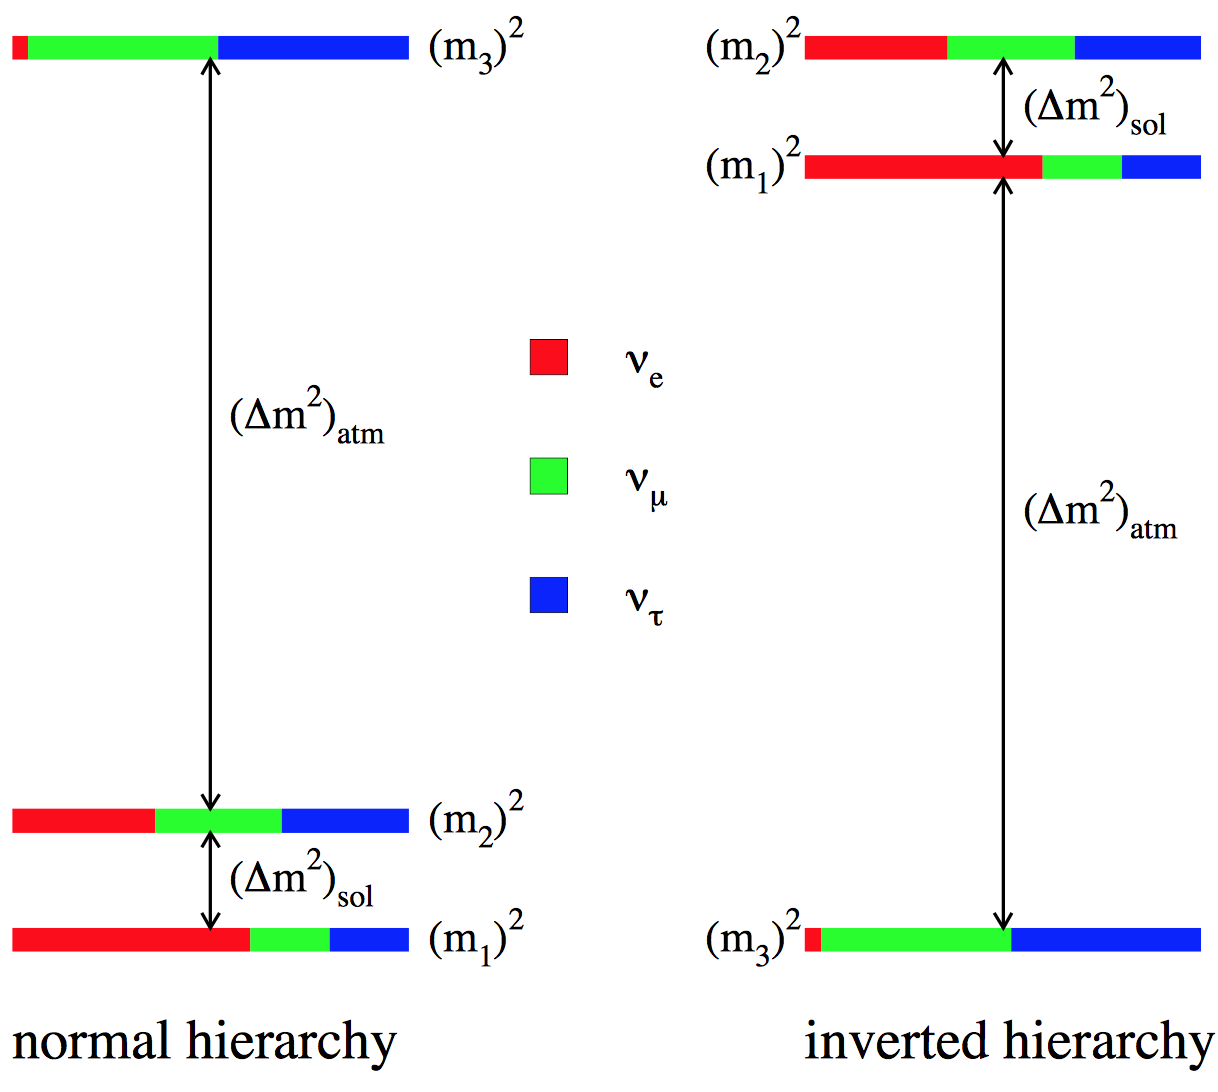
\includegraphics[width=0.5\textwidth]{MassHierarchy}
  \caption[A schematic representation of the two mass hierarchies, showing the fractional components of flavour states in each mass state]
          {A schematic representation of the two mass hierarchies, showing the fractional components of flavour states in each mass state. Left: the normal hierarchy, where the masses are ordered $m_{{1}} < m_{{2}} < m_{{3}}$. Right: the inverted mass hierarchy, where the masses are ordered $m_{{3}} < m_{{1}} < m_{{2}}$. The fractional components of $\nu_{e}$, $\nu_{\mu}$ and $\nu_{\tau}$ are shown in red, green and blue respectively. Figure taken from~\citep{Hewett:2012ns}.}
  \label{fig:Neut_MH}
\end{figure}

%%% Current best limits and overview of exisiting experiments.
\subsection{Current experimental limits, and unanswered questions} \label{sec:Theory_Exp}
There is a large amount of experimental data supporting the oscillation paradigm which has been outlined in Section~\ref{Neut_Oscil}. This is summarised in Table~\ref{tab:NeutProp}~\citep{NuFit2016}, which combines measurements made by many neutrino experiments to produce global fits for the neutrino mixing parameters. \\ 

\begin{table}\centering
  \caption[Three-flavour oscillation parameters from a fit to global data after the NOW-2016 and ICHEP-2016 conferences]
          {Three-flavour oscillation parameters from a fit to global data after the NOW-2016 and ICHEP-2016 conferences. The best fit points (bfp) in the 1st (2nd) column are obtained assuming normal (inverted) ordering, whereas in the 3rd column no ordering is assumed. Note that $\Dmq_{3\ell} \equiv \Dmq_{31} > 0$ for normal ordering, and $\Dmq_{3\ell} \equiv \Dmq_{32} < 0$ for inverted ordering. Table is taken in full from~\citep{NuFit2016}.}
  \label{tab:NeutProp}\resizebox{\columnwidth}{!}{%
    \begin{tabular}{c|cc|cc|c}
      \hline\hline
      & \multicolumn{2}{c|}{Normal Ordering (best fit)}
      & \multicolumn{2}{c|}{Inverted Ordering ($\Delta\chi^2=0.83$)}
      & Any Ordering
      \\
      \hline
      & bfp $\pm 1\sigma$ & $3\sigma$ range
      & bfp $\pm 1\sigma$ & $3\sigma$ range
      & $3\sigma$ range
      \\
      \hline
      \rule{0pt}{4mm}\ignorespaces
      $\sin^2\theta_{12}$
      & $0.306_{-0.012}^{+0.012}$ & $0.271 \to 0.345$
      & $0.306_{-0.012}^{+0.012}$ & $0.271 \to 0.345$
      & $0.271 \to 0.345$
      \\[1mm]
      $\theta_{12} (^{\circ})$
      & $33.56_{-0.75}^{+0.77}$ & $31.38 \to 35.99$
      & $33.56_{-0.75}^{+0.77}$ & $31.38 \to 35.99$
      & $31.38 \to 35.99$
      \\[3mm]
      $\sin^2\theta_{23}$
      & $0.441_{-0.021}^{+0.027}$ & $0.385 \to 0.635$
      & $0.587_{-0.024}^{+0.020}$ & $0.393 \to 0.640$
      & $0.385 \to 0.638$
      \\[1mm]
      $\theta_{23} (^{\circ})$
      & $41.6_{-1.2}^{+1.5}$ & $38.4 \to 52.8$
      & $50.0_{-1.4}^{+1.1}$ & $38.8 \to 53.1$
      & $38.4 \to 53.0$
      \\[3mm]
      $\sin^2\theta_{13}$
      & $0.02166_{-0.00075}^{+0.00075}$ & $0.01934 \to 0.02392$
      & $0.02179_{-0.00076}^{+0.00076}$ & $0.01953 \to 0.02408$
      & $0.01934 \to 0.02397$
      \\[1mm]
      $\theta_{13} (^{\circ})$
      & $8.46_{-0.15}^{+0.15}$ & $7.99 \to 8.90$
      & $8.49_{-0.15}^{+0.15}$ & $8.03 \to 8.93$
      & $7.99 \to 8.91$
      \\[3mm]
      $\delta_\text{CP} (^{\circ})$
      & $261_{-59}^{+51}$ & $\hphantom{00}0 \to 360$
      & $277_{-46}^{+40}$ & $145 \to 391$
      & $\hphantom{00}0 \to 360$
      \\[3mm]
      $\Dmq_{21}\times10^{5} (\eVq)$
      & $7.50_{-0.17}^{+0.19}$ & $7.03 \to 8.09$
      & $7.50_{-0.17}^{+0.19}$ & $7.03 \to 8.09$
      & $7.03 \to 8.09$
      \\[3mm]      
      $\Dmq_{3\ell}\times10^{3} (\eVq)$
      & $+2.524_{-0.040}^{+0.039}$ & $+2.407 \to +2.643$
      & $-2.514_{-0.041}^{+0.038}$ & $-2.635 \to -2.399$
      & $\begin{bmatrix}
        +2.407 \to +2.643\\[-2pt]
        -2.629 \to -2.405
      \end{bmatrix}$
      \\[3mm]
      \hline\hline
    \end{tabular}%
  }
\end{table}

As can be seen from Table~\ref{tab:NeutProp}, the three mixing angles, and the mass squared differences are known to quite high precision. This could lead one to believe that the physics of neutrino oscillation is completely understood, however there are still many questions which remain unanswered. Some of these have already been discussed earlier, and in no particular order are;
\begin{enumerate}
\item \textbf{What is the quadrant of $\theta_{23}$?} As can be seen from Table~\ref{tab:NeutProp}, $\theta_{23}$ is very close to 45$^{\circ}$, representing maximal mixing. However, whether it is more or less than 45$^{\circ}$ remains to be seen.
\item \textbf{What is the value of $\delta_{CP}$?} The value of $\delta_{CP}$ is largely unconstrained to 3$\sigma$, and as discussed in Section~\ref{Neut_Oscil}, the observation of CP violation in neutrinos may help to explain the matter-antimatter asymmetry in the universe.  
\item \textbf{What is the neutrino mass hierarchy?} As discussed in Section~\ref{Neut_Oscil}, though it is known that the $m_{1}$ mass state is lighter than the $m_{2}$ mass state, it is not known whether these are lighter or heavier than the $\nu_{3}$ mass state.
\item \textbf{What is the absolute neutrino mass scale?} The absolute mass of the neutrino is unknown, though cosmological constraints, from Planck CMB data, place an upper limit of $\sum m_{\nu} < 0.23$ eV at the 95\% confidence limit~\citep{Planck}. Neutrino experiments such as KATRIN hope to reach sensitivities of this magnitude by looking for a cut-off in the energy spectrum of $\beta$ decays~\citep{KATRIN}.
\item \textbf{Are neutrinos Dirac or Majorana particles?} This concerns how neutrinos acquire mass, as if they are Dirac particles then they would acquire mass through interactions with the Higgs field, as the other particles in the SM do. However, if they were Majorana particles, then they would acquire at least some of their mass through self-coupling. This would violate lepton number, and mean that neutrinos are their own antiparticle. As discussed in Section~\ref{Neut_Oscil}, experiments are searching for this by looking for neutrinoless double $\beta$ decay.
\item \textbf{Are there sterile neutrinos?} Experimental data from LEP tightly constrains the number of active neutrinos to those predicted by the SM~\citep{LEP}. However, in recent years there have been anomalous results which may hint at so-called sterile neutrinos~\citep{LSND1, LSND2, MiniBooNE}. These sterile neutrinos would not interact, but would still be involved in oscillations. Sterile neutrinos are included in the neutrino mixing formalism by extending the PMNS matrix from a 3 $\times$ 3 matrix, to a (3+N) $\times$ (3+N) matrix, where N is the number of sterile neutrinos. Many short baseline experiments are searching for signatures which would suggest the presence of sterile neutrinos.  
\end{enumerate}
Next generation neutrino experiments, such as DUNE, hope to address some of these unanswered questions. For a review of the experimental aims of DUNE see Section~\ref{sec:DUNEPhys}. \\

%********************************** % Second Section  *************************************
\section{Grand Unified Theories and nucleon decay}  \label{sec:Theory_GUT} %Section - X.2
The subject of Grand Unified Theories (GUTs) is a complicated one and requires a level of mathematics which will not be covered here. However, as Chapter~\ref{chap:FDSims} concerns establishing background limits to nucleon decays, it is necessary to illustrate the basic premise of GUTs and the predictions on nucleon decay which they make, this will be presented in Section~\ref{sec:Theory_NDK}. The mechanism by which cosmic ray muons are able to produce signals which mimic nucleon decays will be presented in Section~\ref{sec:BkNDK}.\\

%********************************** % Third Section  *************************************
\subsection{Overview of grand unified theories} \label{sec:Theory_NDK}  %Section - X.2.3
The basic premise of GUTs is that they attempt to unite the strong, weak and electromagnetic forces. This is achieved by referring to very large energy scales of around 10$^{16}$ GeV~\citep{PhysRevD.25.3092}. One of the first GUTs was that of Georgi and Glashow in 1974, which predicted that the three forces arose from a single interaction based on the SU(5) gauge group~\citep{PhysRevLett.32.438}. One of the things which their theory predicted was that the proton would not be stable, and would have a lifetime $\tau_{p} \simeq 10^{30}$~years. This went against the long-held idea of baryon number conservation, which had been proposed by Weyl to explain why neutrons decayed but protons did not~\citep{Weyl1929}. Proton decay had been considered since Weyl's prediction, but there had never been any prediction of it. One of the earliest limits on the lifetime of the proton had actually been made by Maurice Goldhaber, who noted that if the proton lifetime was less than 10$^{18}$~years we would receive lethal doses of radiation from its decay~\citep{Senjanovic:2009kr}. \\

With the prediction of proton decay, experiments began searching for it in underground labs. The proton lifetime predicted by Georgi and Glashow has now been conclusively ruled out, and inconsistencies have been found with their original theory, such as the gauge couplings not unifying at a common energy, and the neutrinos predicted by it being massless~\citep{Senjanovic:2009kr}. However, it began the search for a GUT, as well as the search for nucleon decay, and so it is interesting from an historical standpoint. Extensions to the original theory have been made which attempt to address some of the issues mentioned above, these extensions predict proton lifetimes of the order $\tau_{p} \leq 10^{35}$~years~\citep{Foot1989, Dorsner:2005fq}. \\

SUperSymmetry (SUSY) is an extension of the standard model which aims to to rectify many of the inconsistencies seen in the SU(5) models. It does this by predicting that there are ``superpartners'' to the bosons and fermions predicted by the SM, which differ from their SM counterparts by a spin factor of $\frac{1}{2}\hbar$. An ``s'' is added to the names of the SM fermions (sup, selectron), and ``ino'' is added to the names of the SM bosons (wino, gluino), to denote the difference between SM particles and their superpartners~\citep{Martin:1997ns}. The Minimally Supersymmetric Standard Model (MSSM) is the simplest SUSY theory and it predicts a single superpartner to each of the known SM fermions and bosons~\citep{Castano:1993ri}. Supersymmetric SU(5) models have been popular for many years and even predicted the value of the Weinberg angle and that the top quark would have a mass of around 200 GeV~\citep{Senjanovic:2009kr}. Though the initial proton lifetimes of $\tau_{p} \simeq 10^{30-31}$~years have now been ruled out, it is possible to get proton lifetimes of $\tau_{p} \simeq 10^{34-36}$~years, which are well within the current experimental limits~\citep{Gomez:1999kv}. \\

In the MSSM it is possible to have proton decay lifetimes of less than 1~s, through baryon and lepton number violating interactions, unless a symmetry called $R$-parity~\citep{FARRAR1978575} is introduced (Equation~\ref{eq:RParity}).
\begin{equation}
  \label{eq:RParity}
  P_{R} = (-1)^{3(B-L)+2s}
\end{equation}
where $B$ is baryon number, $L$ is lepton number, and $s$ is spin. SM particles have $R$ parity +1, whilst supersymmetric particles have $R$-parity -1. The baryon - lepton number ($B-L$) is generally conserved in GUTs, as a result of $R$-parity. However, in order to explain neutrino mass and mixing, $R$-parity must be broken~\citep{Senjanovic:2009kr}. This has the unfortunate consequence of making the lightest neutralino unstable, meaning that it cannot be the Lightest Supersymmetric Particle (LSP), as it would decay too quickly to explain dark matter. This then means that the best candidate for the LSP is the unstable gravitino~\citep{Senjanovic:2009kr}. However, after allowing for $R$-parity to be broken, additional channels of nucleon decay become possible, such as $n \rightarrow K^{+} + l^{-}$ and $p \rightarrow K^{+} + l^{-} + \pi^{+}$. Chapter~\ref{chap:FDSims} will concern simulations of the muon-induced background to the $n \rightarrow K^{+} + e^{-}$ decay channel, this decay was first proposed by invoking the non-conservation of $B-L$~\citep{PATI1983330, PhysRevLett.44.1316}. As will be shown in Table~\ref{tab:NDKLim}, the current lifetime limit on this channel is 3.2$\times$10$^{31}$~years~\citep{berger:in2p3-00015565}. It can be shown that the decay rate of the $n \rightarrow K^{+} + l^{-}$ channel may be an order of magnitude larger than that of the proton~\citep{Senjanovic:2009kr, Vissani:1995hp}. All decay channels which do not non-conserve $B-L$ currently have very low limits on their lifetimes~\citep{PDGReview} and so warrant further study, as nucleon decay signatures may potentially be observed with relatively low lifetimes. \\

Finally, it is also possible to construct GUTs which use higher order gauge groups, such as the SO(10) group. When considering SO(10) theories, supersymmetric models are normally considered, as ordinary SO(10) models have failed to be able to predict fermion masses and mixings~\citep{Senjanovic:2009kr}. However, the supersymmetric models are able to accommodate right handed neutrinos, explain the disparity between the quark and lepton mixing angles at SM energies, and predict the branching ratios of proton decays. As such, predictions of the proton lifetimes of the order of 10$^{33-36}$~years exist, with an upper limit of 10$^{38}$~years in the $p \rightarrow K^{+} \overline{\nu}$ decay channel~\citep{Severson:2015dta}. \\

Over the years there have been many experiments which have searched for the signatures of nucleon decay, these have included NUSEX~\citep{BATTISTONI1983454}, FREJUS~\citep{berger:in2p3-00015565}, Soudan I/II~\citep{SoudanLim}, and IMB~\citep{Gajewski:1989gh}. The current experimental limit on the proton lifetime is held by the SK experiment, which sets a lower limit on partial lifetime in the $p\ensuremath{\rightarrow}{e}^{+}{\ensuremath{\pi}}^{0}$ decay mode of 1.6 $\times$ 10$^{34}$~years~\citep{PhysRevD.95.012004}. A successor to SK, called Hyper-Kamiokande (HK), is planned for the mid 2020s~\citep{Abe:2011ts} and will increase the proton decay lifetime sensitivity by around an order of magnitude. DUNE will also search for nucleon decays, and will have a sensitivity to a number of nucleon decay modes which competes with HK despite being much smaller, due to the increased resolution of LArTPCs as compared to water Cherenkov detectors. The sensitivity of DUNE to nucleon decay will be discussed in Section~\ref{sec:DUNE_NDK}. \\  

%********************************** % Third Section  *************************************
\subsection{Backgrounds to nucleon decay} \label{sec:BkNDK}  %Section - X.2.3
In order to observe such rare processes it is necessary to place experiments in environments which have as little background as possible. For this reason, experiments which search for proton decay are placed far below the Earth's surface to reduce the cosmic ray flux. Such searches would be impossible if they were attempted on the Earth's surface. At large depths the hadronic flux is totally suppressed, however cosmic ray muons can survive to depths of over a mile underground. These high energy cosmic muons are able to produce signal mimicking events in underground detectors. Therefore, to observe the signal from a nucleon decay, these events have to be identified and rejected. \\

In the discussion of backgrounds to nucleon decay, reference will be given to the $p \rightarrow K^{+} \overline{\nu}$ decay channel, where the signal is a lone $K^{+}$ in the detector. The kaon is isolated as the neutrino will not interact before escaping the detector, and the recoiling nucleus would have too little energy to be detected. Though it is difficult to imagine a situation where a cosmic muon would directly produce an isolated kaon in the detector, one of its interaction products could do so. For instance, a muon could produce a $K^{0}_{L}$ outside of the detector, which then propagates into the detector, and undergoes charge exchange with a proton in the nucleus of an argon atom. This would produce an isolated kaon inside the TPC, with no associated tracks coming from outside the detector (the $K^{0}_{L}$ is neutral and so does not produce a track in LArTPCs). This event structure would look very similar to a nucleon decay event, and a schematic of such an interaction is shown in Figure~\ref{fig:K0LongBackground}. It is important to note that as LArTPCs are not magnetised it is very difficult to discern the charge of a kaon, and so a $K^{\pm}$ are largely indistinguishable. \\

\begin{figure}
  \centering
  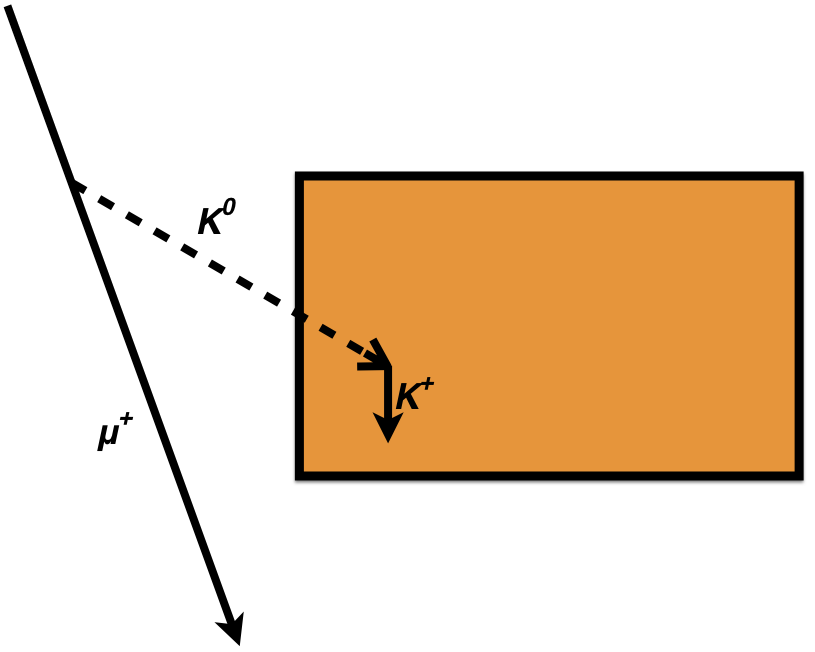
\includegraphics[width=0.5\textwidth]{KaonNDKInteraction}
  \caption[Schematic of a muon event mimicking a nucleon decay]
          {Schematic of a muon event mimicking a nucleon decay. A cosmic muon produces a $K^{0}_{L}$ outside of the detector volume, which then interacts producing an isolated kaon. There would be no other charged tracks produced, and so the event would be indistinguishable from a real proton decay event.}
  \label{fig:K0LongBackground}
\end{figure}

Atmospheric neutrinos are also able to produce signals which mimic nucleon decays if they interact within the active volume. The simulations described in Chapter~\ref{chap:FDSims} concern backgrounds induced by cosmic ray muons. The backgrounds induced by atmospheric neutrinos will not be considered in this thesis. \\

Though background inducing events like the one shown in Figure~\ref{fig:K0LongBackground} are rare, the nucleon decay rate is very low, and so it is necessary to identify background events and reject them when searching for a signal. For this reason a fiducial cut is often applied, as many of the $K^{0}_{L}$s will interact close to the detector edge. Should an interaction pass this cut, it is possible to apply strict energy criteria to the reconstructed energies. This is because the energies of the particles produced in a nucleon decay event are well defined. This will be discussed further in Chapter~\ref{chap:FDSims} in the context of the $n \rightarrow K^{+} e^{-}$ decay channel. In the case of the $p \rightarrow K^{+} \overline{\nu}$ decay channel, one would expect the kaon to have a momentum of about 340 MeV, and a total energy of about 600 MeV. The kaon would also be expected to decay at rest, and so the decay products from the kaon should have an energy equal to the rest mass of the kaon (493.677 MeV~\citep{PDGReview}). The derivation of how these energies are calculated will be shown in Section~\ref{sec:NDKKin}, with reference to the $n \rightarrow K^{+} e^{-}$ decay channel. \\
